\chapter{GUI Design}
\thispagestyle{plain}

This chapter describes the basic structure of the instance builder web page and the various assertions and conditions required for a well defined scheduling instance.

\section{Instance structure}
To facilitate compatibility with backend C++ code, the JavaScript instance object is converted to a JSON string. JSON (JavaScript Object Notation) is a text format that is completely language independent but uses conventions that are familiar to many different programming languages, including C, C++, Java, JavaScript, Python and others. These properties make JSON an ideal data-interchange format.

JSON is built on two universal data structures:
\begin{itemize}
\item A collection of name/value pairs. In various languages, this is realized as an object, record, struct, dictionary, hash table, keyed list, or associative array.
\item An ordered list of values. In most languages, this is realized as an array, vector, list, or sequence.
\end{itemize}
Virtually all programming languages support these structures in one form or other. In JSON, they take on these forms:

An \emph{object} is an unordered set of name/value pairs. An object begins with \{ (left brace) and ends with \}  (right brace). Each name is followed by \lstinline{:} (colon) and the name/value pairs are separated by \lstinline{,} (comma).
\section{Instance object}
\label{instanceCompletion}
\begin{figure}[htbp]
\begin{center}
\begin{lstlisting}[xleftmargin=.2\textwidth, xrightmargin=.2\textwidth]
{
	"Name": "Scheduling_Instance",
	"Horizon": 8,
	"Units": [],
	"States": [],
	"Orders": [],
	"Utilities": [],
	"Tasks": [],
	"isCompleteInstance": false
}
\end{lstlisting}\end{center}•
\caption{Instance JSON}
\label{code:Instance}
\end{figure}•
The structure of the Instance JSON object is as shown in Figure \ref{code:Instance}. The empty arrays \lstinline{[]} for \lstinline{"Units"}, \lstinline{"States"}, \lstinline{"Tasks"}, \lstinline{"Utilities"} and \lstinline{"Orders"} in the structure contain the JSON objects as specific to the instance. \lstinline{"Name"} is a string denoting the given name for the instance. \lstinline{"Horizon"} is an integer or float. \lstinline{"isCompleteInstance"} is a boolean \lstinline{true} or \lstinline{false} value denoting if an instance is completely specified.

Figures \ref{fig:unitJSON} - \ref{fig:taskJSON} show the structures of the unit, state, utility, order and task JSON objects respectively.
\begin{figure}[!tbp]
  \centering
  \begin{minipage}[b]{0.4\textwidth}
    \begin{lstlisting}
{
	"Name": "Unit1",
	"MaximumCapacity": 100
}
\end{lstlisting}
    \caption{Unit JSON object}
\label{fig:unitJSON}
  \end{minipage}
  \hfill
  \begin{minipage}[b]{0.4\textwidth}
    \begin{lstlisting}
{
	"StateName": "State1",
	"StateInitialLevel": 100,
	"StateMaxLevel": 100,
	"IsZeroWait": true,
	"IsUIS": false,
	"Price": 10
}
\end{lstlisting}
    \caption{State JSON object}
  \end{minipage}
\end{figure}

\begin{figure}[!tbp]
  \centering
  \begin{minipage}[b]{0.4\textwidth}
\begin{lstlisting}
{
	"Name": "Utility1",
	"MaximumAvailability": 250
}
\end{lstlisting}
    \caption{Utility JSON object}
\label{fig:utilityJSON}
  \end{minipage}
  \hfill
  \begin{minipage}[b]{0.4\textwidth}
\begin{lstlisting}
{
	"StateName": "Product1",
	"Amount": 100
}
\end{lstlisting}
    \caption{Order (demand) JSON object}
  \end{minipage}
\end{figure}

An instance is deemed `complete' if:
\begin{enumerate}
\item At least one valid unit
\begin{itemize}
\item Positive maximum capacity
\end{itemize}
\item At least two states
\begin{itemize}
\item Non-negative maximum capacity
\item Initial level is less than or equal to maximum capacity
\item At least one state with positive initial level
\end{itemize}
\item At least one valid task
\begin{itemize}
\item At least one compatible unit with non-zero processing time (at least one of $\alpha$ or $\beta$ is non-zero)
\item At least one consumed state
\item At least one produced state
\end{itemize}
\item Positive horizon and at least one state to be sold with positive price OR At least one state in demand with positive demand amount
\end{enumerate}



%\subsection{Tasks}
\begin{figure}[htbp]

\begin{lstlisting}[xleftmargin=.2\textwidth, xrightmargin=.2\textwidth]
{
	"TaskName": "Task1",
	"CompatibleUnits": [
		{
		"UnitName": "Unit1",
		"alpha": 5,
		"beta": 1
		}
	],
	"ConsumedStates": [
		{
		"ConStateName": "State1",
		"consRatio": 1
		}
	],
	"ProducedStates": [
		{
		"ProdStateName": "State2",
		"prodRatio": 1
		}
	],
	"ConsumedUtilities": [
		{
		"ConsUtilName": "Utility1",
		"CompUnit": "Unit1",
		"gamma": 2,
		"delta": 0.2
		}
	]
}
\end{lstlisting}
\caption{Task JSON object}
\label{fig:taskJSON}
\end{figure}•


\section{Overall scheduling process flow}
\begin{figure}[htbp]
\centering
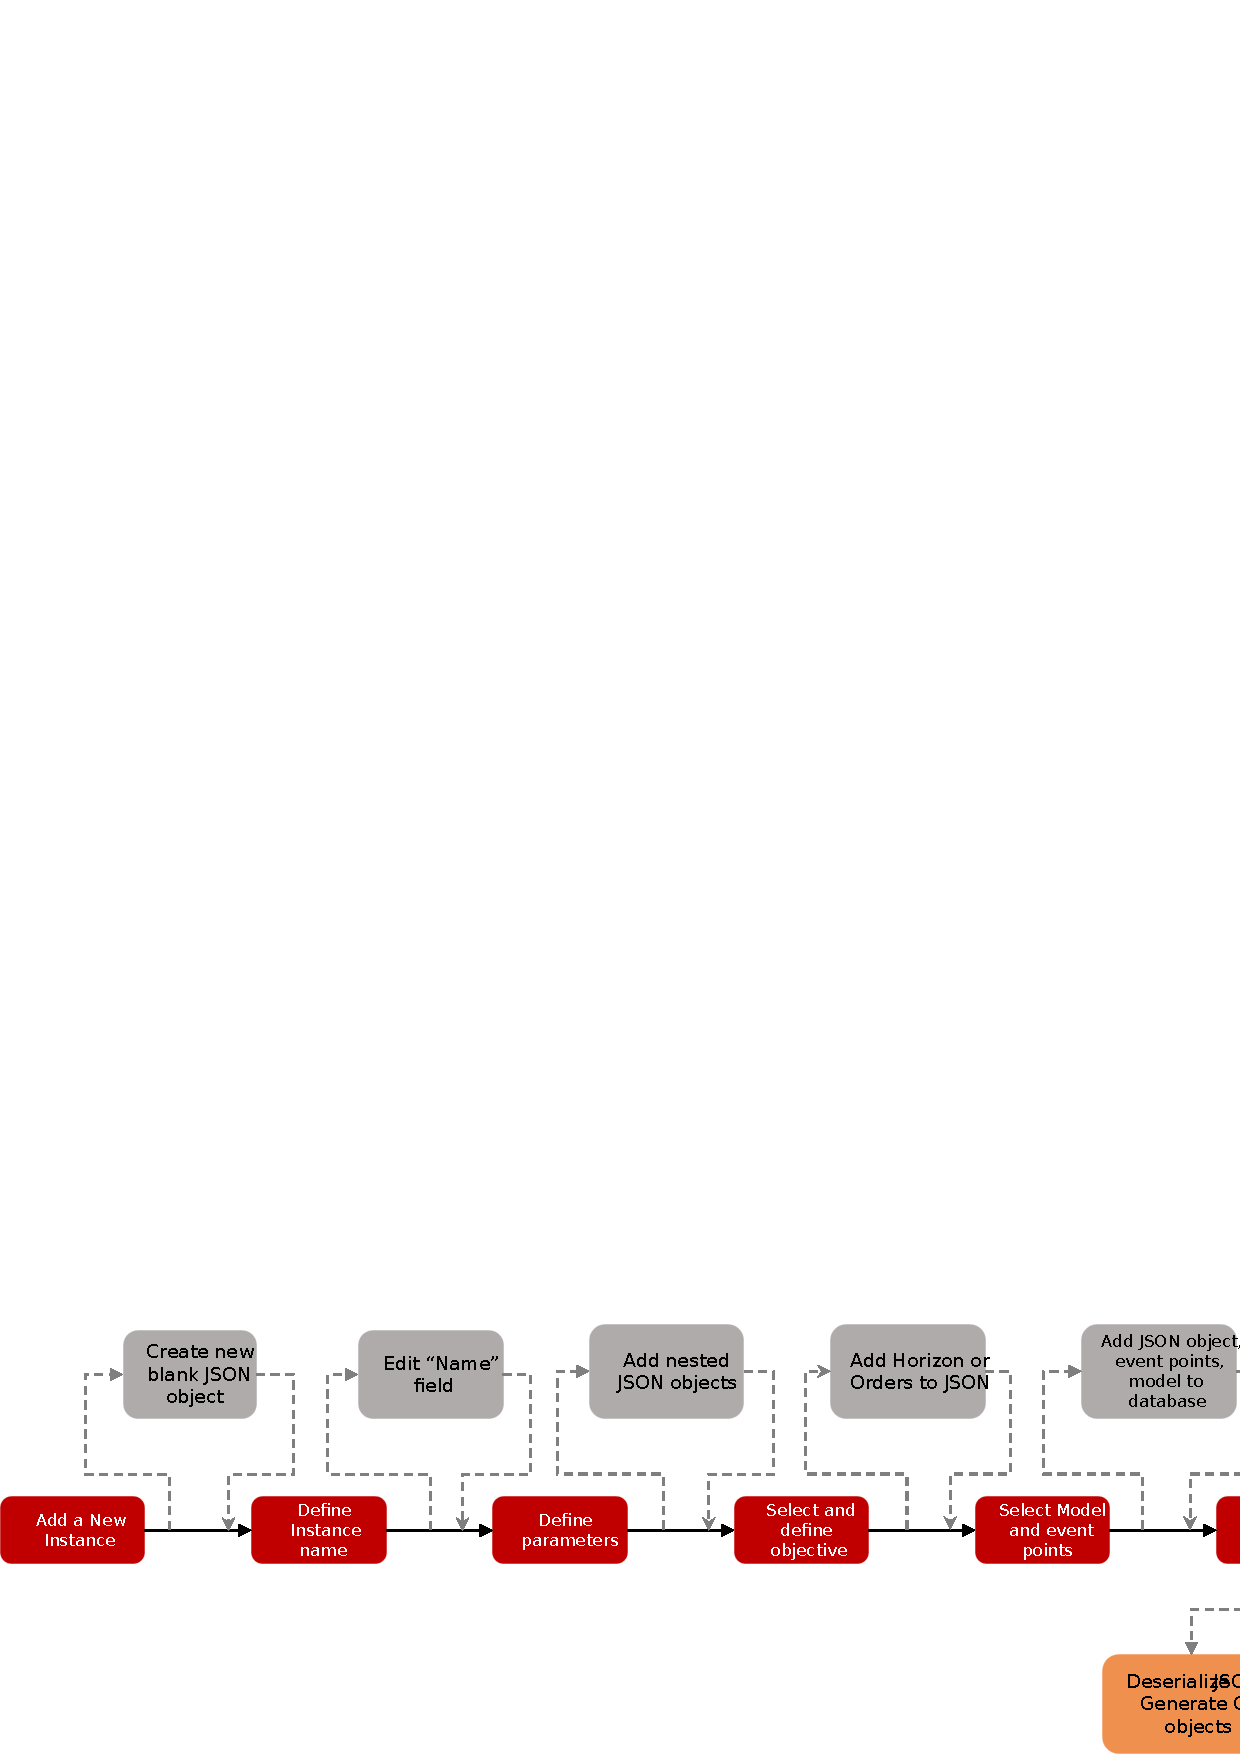
\includegraphics[width=\linewidth]{Images/Communication.png}
\caption{Overall process flow}
\label{fig:Communication}
\end{figure}

Figure \ref{fig:Communication} shows the underlying process behind creating and submitting a scheduling instance. At each stage of the instance building process, the JSON object is converted to a string by means of the \texttt{JSON.stringify()} method in JavaScript and saved in a backend mySQL database. A more detailed process flow for parameter and objective input is shown in Fig. \ref{fig:paraminput}. Once the the instance is complete and amenable to optimization, in the deterministic version, the user has the option of selecting the number of event points and scheduling model to be used. In the uncertain version, the user has additional choices to select uncertain parameters and adjustable variables.

\begin{figure}[htbp]
\centering
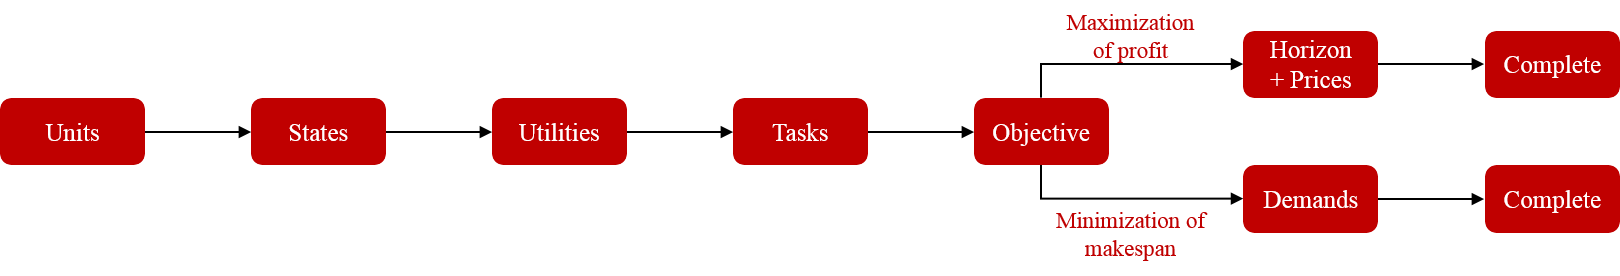
\includegraphics[width=\linewidth]{Images/ParameterObjectiveInput.png}
\caption{Parameter and objective input}
\label{fig:paraminput}
\end{figure}

On submitting, a C++ JSON deserializer converts the JSON string to C++ objects. These are then used to build a mixed-integer model in CPLEX according to the model specified by the user.

On successful completion, the following statistics are displayed on the results page:
\begin{itemize}
\item Run time
\item Forumlation
\item Number of event points
\item Objective type
\item Solver status
\item Objective value
\item Number of constraints
\item Number of binary variables
\item Number of continuous variables
\item Number of continuous variables
\item Nodes
\item Root node relaxation
\item Relative gap (\%)
\end{itemize}

If the user has elected to incorporate uncertainty into the instance, the following additional information is displayed:
\begin{itemize}
\item Uncertain Parameter(s)
\item Level of uncertainty
\item Adjustable Variable(s)
\end{itemize}

Additionally, a Gantt chart for the optimal schedule and material inventory charts are displayed. If utilities are specified by the user, then a utility consumption plot is also displayed.

\section{Instance builder}

\begin{figure}[htbp]
\centering
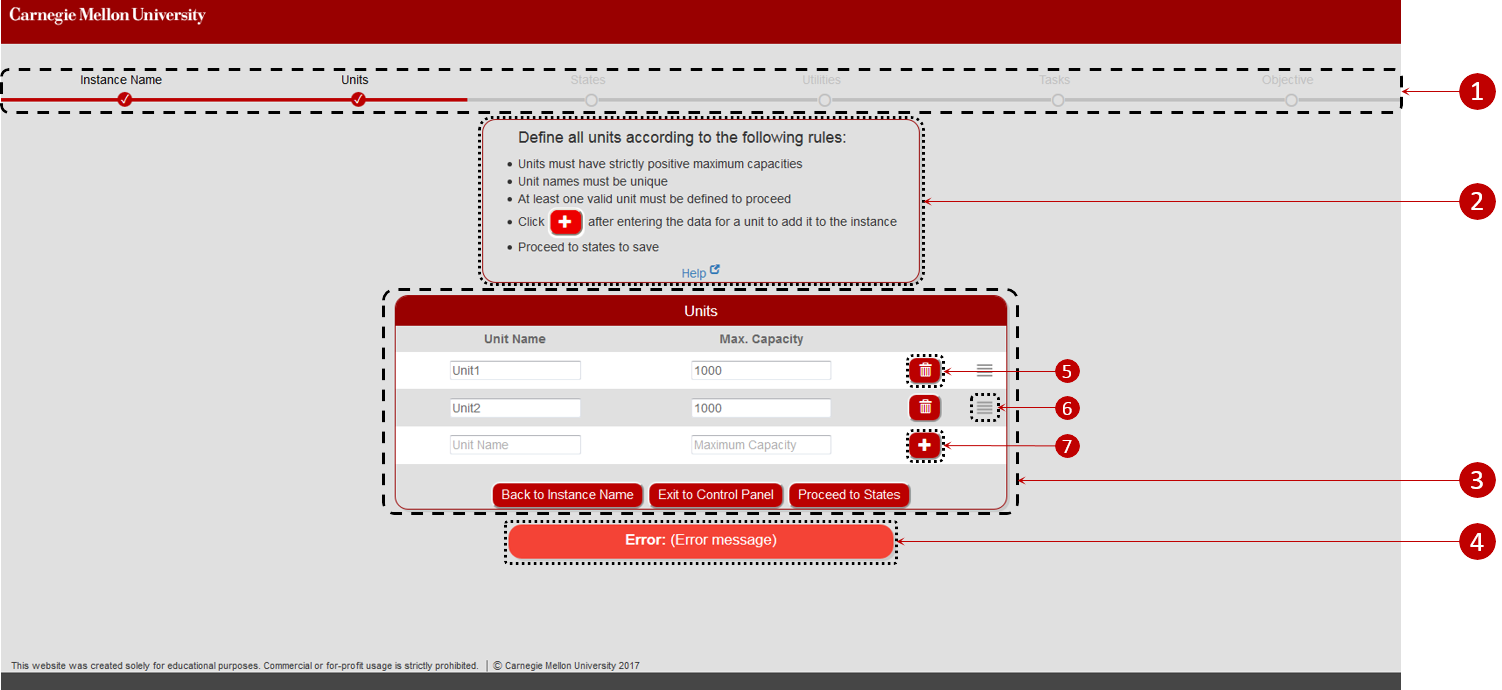
\includegraphics[width=\linewidth]{Images/GUIDesign.png}
\caption[Instance builder elements]{Instance builder elements:
1. Progress bar
2. Instructions
3. Input table
4. Error message(s)
5. Delete item 
6. Drag and drop to rearrange
7. Add new item}
\label{fig:IBGUI}
\end{figure}

Figure \ref{fig:IBGUI} shows the elements in the instance builder GUI. The screenshot in the figure shows the elements in the Units input table. The structure of the States, Utility and Tasks input table follows the same structure. A progress tracker is provided to track the status of the instance being edited. 

Error messages are displayed to ensure that the user input is valid and the instance completion criteria listed in section \ref{instanceCompletion} are satisfied.
 Once a particular set of inputs is completed, clicking on the proceed button will display the next input table.






\section{Submission page}

\begin{figure}[htb]
\centering
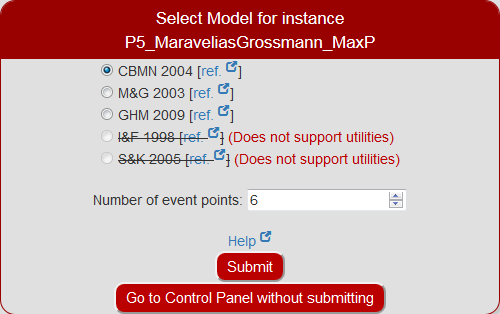
\includegraphics[width=0.8\linewidth]{Images/SelectModelUtilities.png}
\caption{Model selection table for an instance involving utilities}
\label{fig:selectModel}
\end{figure}

On successful completion, an instance becomes available for submission. A screenshot of the model selection table is shown in Fig. \ref{fig:selectModel}. The CBMN 2004 model is selected by default for both the deterministic and uncertain versions. The I\&F 1998 and S\&K 2005 models do not support instances with utilities involved.

\subsection{Uncertainty frameworks}

If the user elects to incorporate uncertainty in the instance, four types of uncertain variables are available:
\begin{enumerate}
\item Fixed processing time ($\alpha$)
\item Fixed and variable processing time ($\alpha + \beta$)
\item Task yield ($\rho_p$)
\item Fixed processing time and task yield ($\alpha + \rho_p$)
\end{enumerate}

The availability of SRO and ARO frameworks for each of the sets of uncertain variables is shown in Table \ref{tab:adjvars}. If ARO is selected, the uncertain parameters selected dictate the availability of adjustable variables.

\begin{table}[htb]
\centering
\caption{Uncertainty frameworks and  adjustable variables}
\label{tab:adjvars}
\begin{tabular}{@{}cccccc@{}}
\toprule
                  & \multicolumn{2}{c}{Frameworks} & \multicolumn{3}{c}{Adjustable variables} \\ \cmidrule(l){2-6} 
Uncertain parameters   & SRO        & ARO        & \phantom{S } T \phantom{ S}            & \phantom{S } S \phantom{ S}           & B + S       \\ \midrule
$\alpha$          & \checkmark & \checkmark & \checkmark   & \xmark      & \checkmark  \\
$\alpha + \beta$  & \checkmark & \checkmark & \checkmark   & \xmark      & \xmark      \\
$\rho_p$          & \xmark     & \checkmark & \xmark       & \checkmark  & \xmark      \\
$\alpha + \rho_p$ & \xmark     & \checkmark & \checkmark   & \checkmark  & \xmark      \\ \bottomrule
\end{tabular}
\end{table}